\documentclass{standalone}
\usepackage{tikz}
\usepackage{ctex,siunitx}
\usepackage{tkz-euclide}
\usepackage{amsmath}
\usetikzlibrary{patterns, calc}
\usetikzlibrary {decorations.pathmorphing, decorations.pathreplacing, decorations.shapes,}
\begin{document}
\small
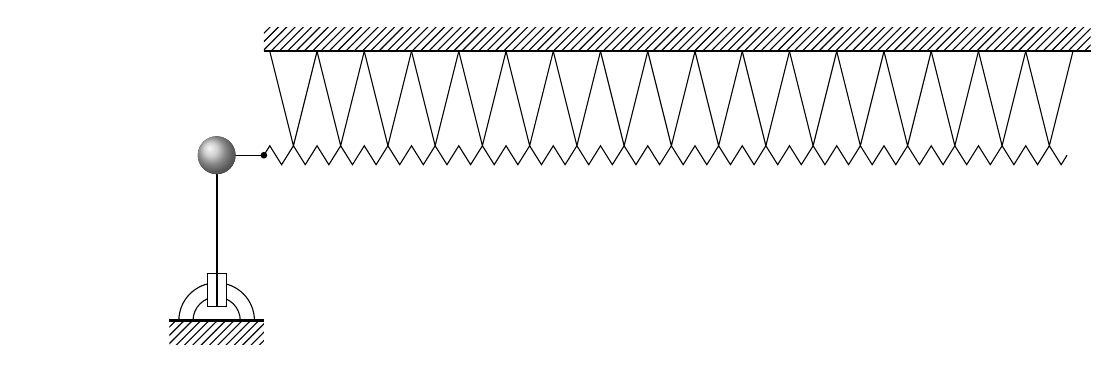
\begin{tikzpicture}[>=stealth,scale=0.6]
  \useasboundingbox(-5.0,2.7)rectangle(17.5,-4);
  % \node at (-2.5,0)[left]{$t=0$};
  \fill(0,0)circle(2pt);
  \draw(0,0)--++(-1,0);
  \draw(-1.5,-3.5)arc(180:0:0.5)(-1.8,-3.5)arc(180:0:0.8);
  \draw[fill=white](-1.2,-2.5)rectangle(-0.8,-3.2);
  \draw[thick](-1,0)--++(0,-3.2)(-2,-3.5)--(0,-3.5);
  \fill[pattern=north east lines](-2,-3.5)rectangle(0,-4);
  \fill[ball color=lightgray] (-1,0)circle(0.4);
  \foreach \x in {0,1,...,16}
    { \draw(\x,0)--++(0.125,0.2)--++(0.25,-0.4)--++(0.25,0.4)--++(0.25,-0.4)--++(0.125,0.2); }
  \foreach \x in {0.625,1.625,...,17}
    { \draw(\x,0.2)--(\x-0.5,2.2)(\x,0.2)--(\x+0.5,2.2); }
  \fill[pattern=north east lines,](0,2.2)rectangle(17.5,2.7);
  \draw[thick](0,2.2)--(17.5,2.2);
\end{tikzpicture}
\end{document}